\documentclass[a4paper, 10pt]{article}
\usepackage{amsmath}
\usepackage{amssymb}
\usepackage[justification=raggedright,singlelinecheck=false]{caption}
\usepackage{graphicx}
\usepackage{float}
\usepackage[margin=0.75in]{geometry}
\usepackage{hyperref}
\usepackage{subcaption}
\usepackage{tabularx}

\title{Gaussian Processes for Time Series}
\date{\today}
\author{Raphaela Azar and Sbonelo Gumede \\
Supervised by Prof. Birgit Erni\\
The University of Cape Town}

\begin{document}

   \maketitle

   \begin{flushleft}
   
   \section*{Introduction}

   In this paper we hope to define what is a Gaussian process. How can you use a Gaussian process for time series analysis? Compare the peformance of a Gaussian process to other time series analysis models such as state-space models. An area of application included is predicting the level of air pollution in the Table View station in Cape Town for the year of 2019. Another area of application is predicting the gold price for South Africa for the year of 2020. This is done in a Bayesian framework in order to make probabilistic statements and obtain a predictive distribution for future forecasts.

   \vspace{1em}

   A Gaussian process is a stochastic process denoted by $\{X_{t} \}_{t \in \mathcal{I}}$, where the parameter space $\mathcal{I}$ and the state space $\mathcal{U}$ are real numbers. 
   At each point $t \in \mathcal{I}$, the state $X_{t} \sim \mathcal{N}(f(x_{t}), \, g(x_{t}))$, where $f(x_{t})$ is a mean function and $g(x_{t}) \geq 0$ is the covariance function.  
   Consider a simple example shown in figure 1, where $f(x_{t}) = x_{t} + e, \, \text{where} \, e \sim \mathcal{N}(0, 1) \, \text{and} \, g(x_{t}) = 1 + \text{sin}^{2}(x_{t})$.
   
   \begin{figure}[H]
            \raggedright
            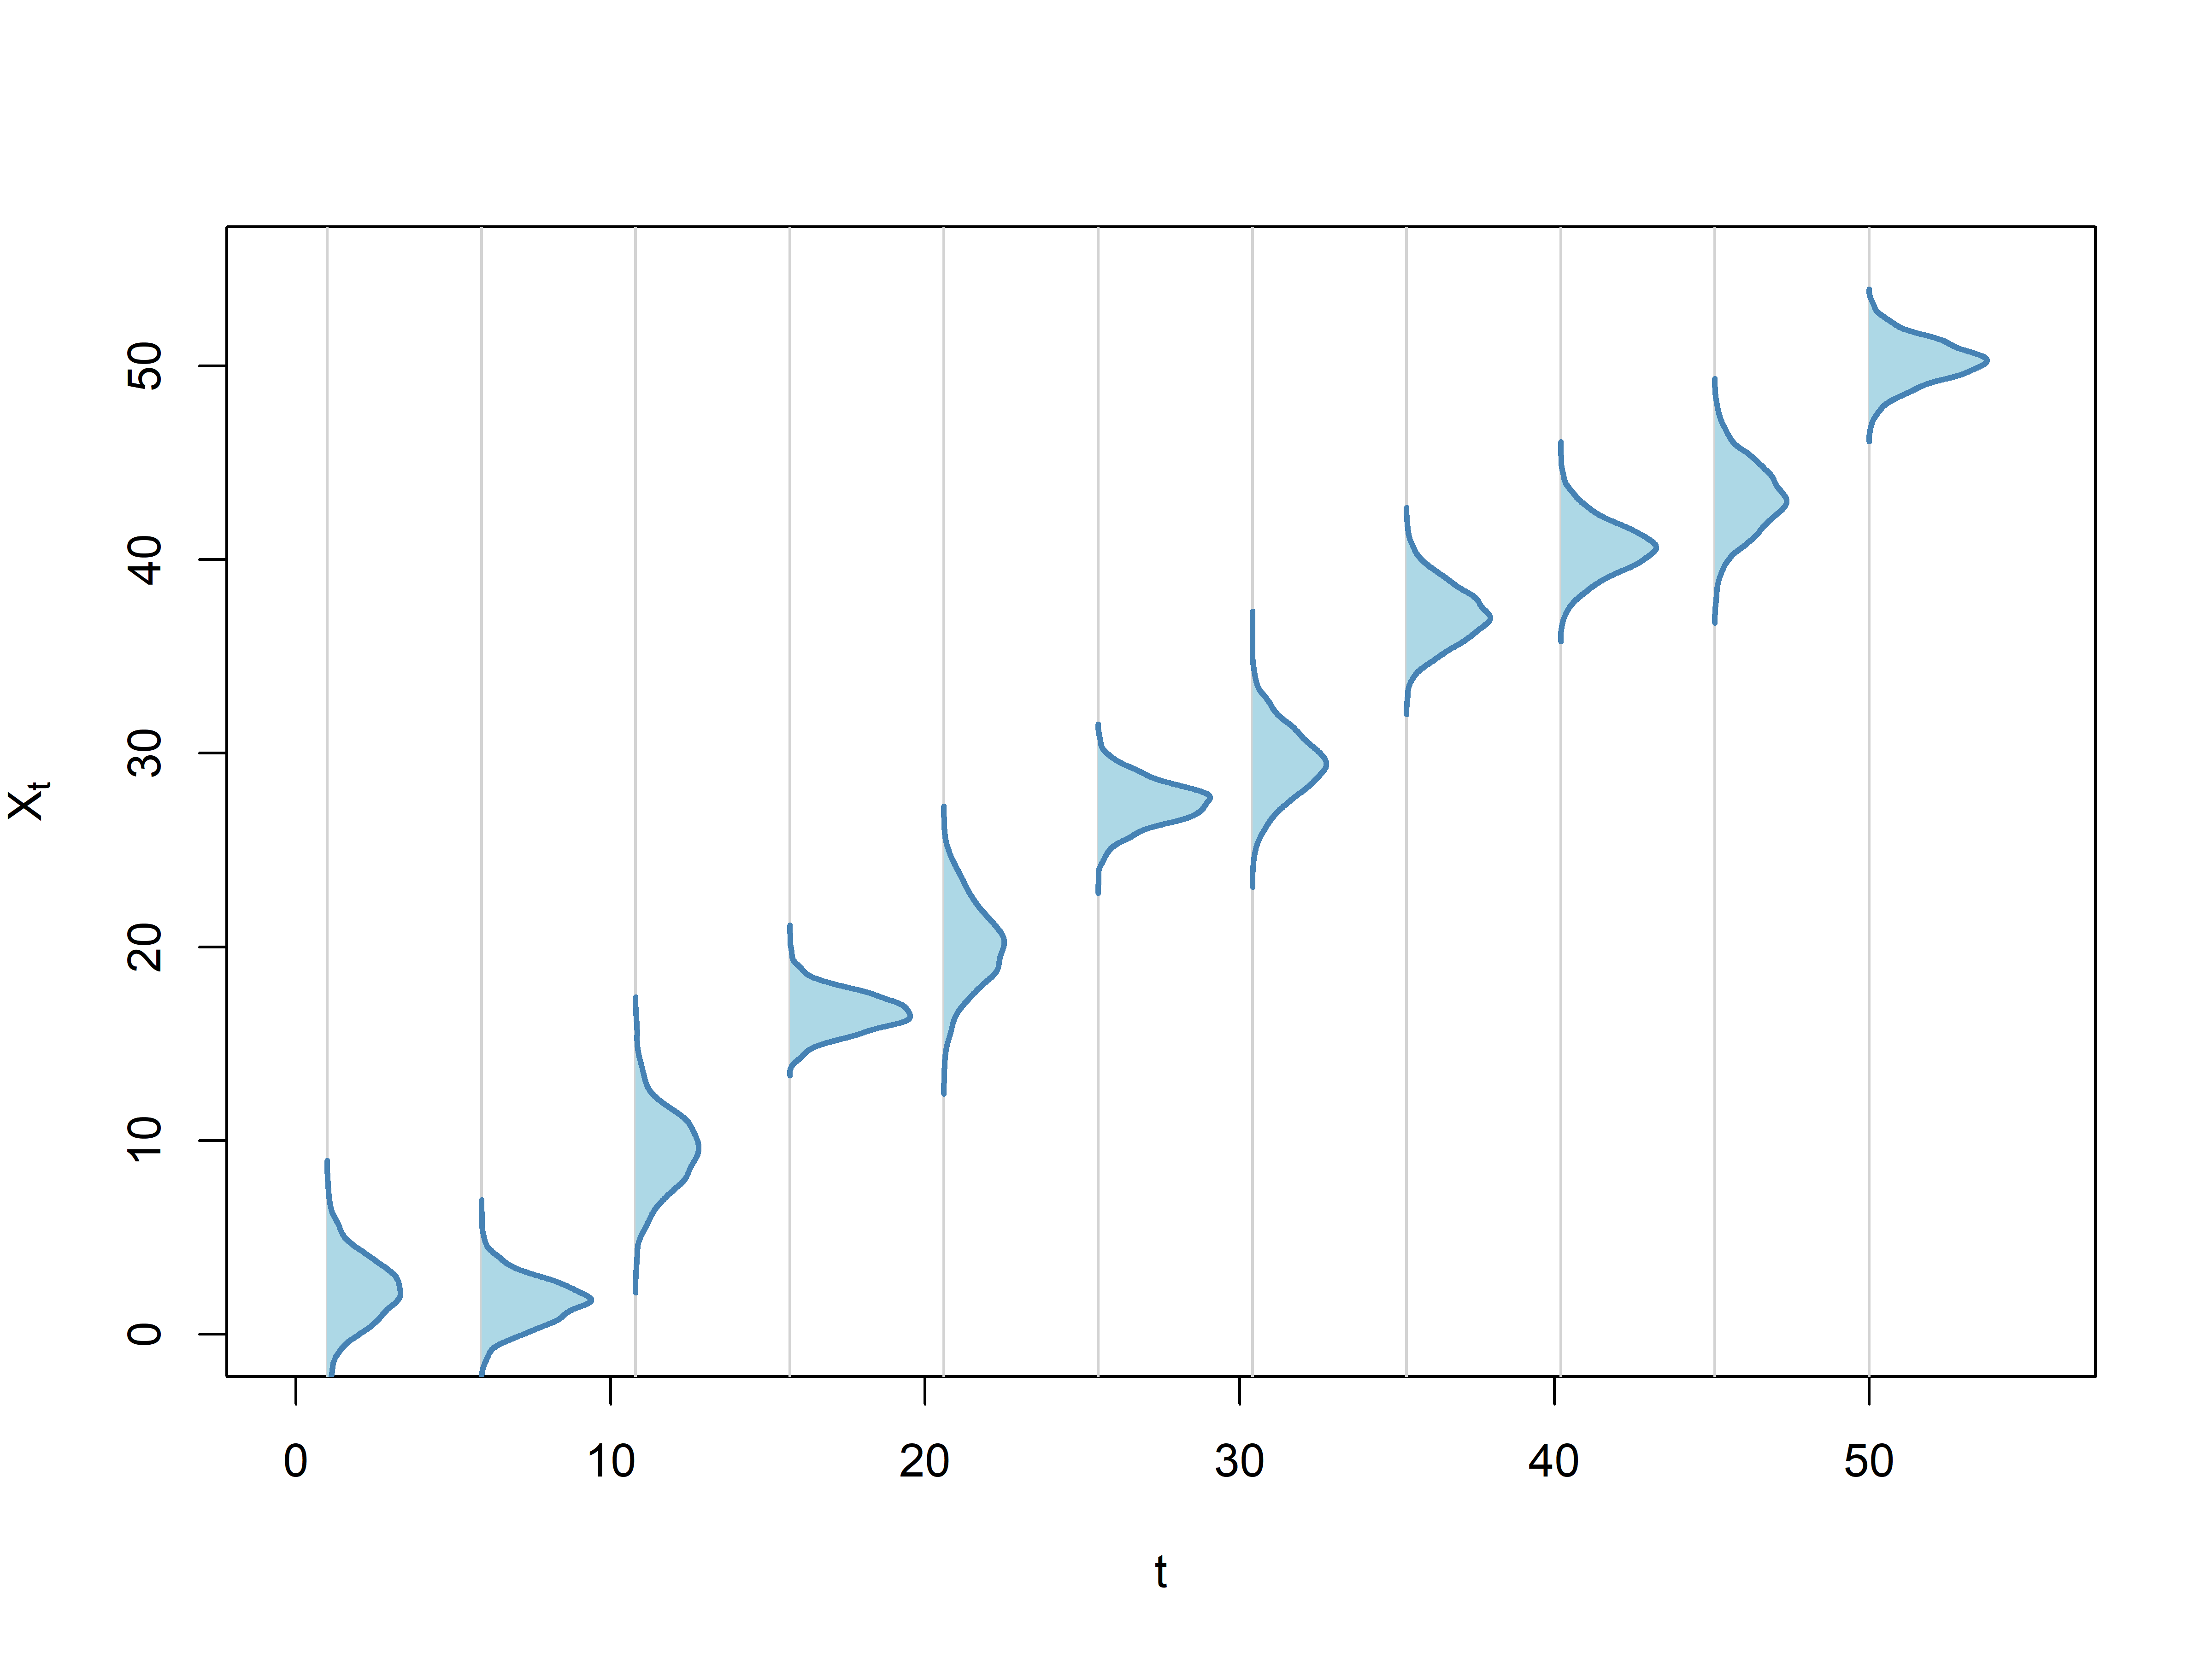
\includegraphics[width=0.48\linewidth]{../images/gp.png}
            \caption{An example of a Gaussian process.}
   \end{figure}
   
   A special property of Gaussian processes is that if you take a countable finite set of observations $\{x_{1}, \, \ldots, \, x_{p}\}$ their joint distribution is 
   $
   \mathbf{X} =
   \begin{bmatrix}
      X_{1} \\
      \vdots \\
      X_{p}
   \end{bmatrix}
   \:
   \sim \mathcal{N}_{p}(\boldsymbol{\mu}, \, \boldsymbol{\Sigma}),
   \:
   \text{where}
   \:
   \boldsymbol{\mu} = 
   \begin{bmatrix}
      f(x_{1}) \\
      f(x_{2}) \\
      \vdots \\
      f(x_{p})
   \end{bmatrix}  
   \: 
   \text{and}
   \:
   \boldsymbol{\Sigma} = 
   \begin{bmatrix}
      g(x_{1}, \, x_{1}) & g(x_{1}, \, x_{2}) & \cdots & g(x_{1}, \, x_{p}) \\
      g(x_{2}, \, x_{1}) & g(x_{2}, \, x_{2}) & \cdots & g(x_{2}, \, x_{p}) \\
      \vdots & \vdots & \ddots & \vdots \\
      g(x_{p}, \, x_{1}) & g(x_{p}, \, x_{2}) & \cdots & g(x_{p}, \, x_{p})
   \end{bmatrix}$.

   \vspace{1em}
   
   Often in the literature people use $f(x_{t}) = 0$ and $g(x_{i}, \, x_{j}) = \alpha^{2} \text{exp}(- \frac{1}{2} (\frac{|x_i - x_j|}{\rho})^2) + \sigma\delta_{ij}$, where $\alpha$ and $\rho$ are hyperparameters and $\delta_{ij}$ is an indicator function. The latter is known as the squared-exponential kernel. Some kernel functions common in the literature are the following:

   \vspace{1em}
   
   There are two ways of modeling time series data. The first one is functional mapping $y = f(x) + e$, where $y$ is the response variable, $x$ is the explanatory variable, and $e$ is typically white additive noise. The noise is assumed to be uncorrelated with one another. Although the simplicity of functional mapping is attractive, functional mapping neglects the time component rendering it useless for our purposes. The second one is curve fitting, where $x$ is often time and $y$ is the response variable. This is ideal for our purposes since we are accounting for the time dependence between successive observations.

   \section*{Air pollution example}
   \subsection*{Exploratory data analysis}
   
      \begin{table}[H]
         \raggedright
         \begin{tabularx}{\textwidth}{|l|l|X|l|}
         \hline
         \text{Variable} & \text{Name} & \text{Description} & \text{Unit} \\
         \hline
         \(\text{NO}_{2}\) & Nitrogen dioxide & A harmful gas from vehicles and industry. & \(\mu\text{g}/\text{m}^{3}\) \\
         \hline
         \(\text{PM}_{10}\) & Particulate matter 10 & Small inhalable dust particles. & \(\mu\text{g}/\text{m}^{3}\) \\
         \hline
         \(\text{SO}_{2}\) & Sulphur dioxide & Mainly from burning fossil fuels. & \(\mu\text{g}/\text{m}^{3}\) \\
         \hline
         Speed & Wind speed & How fast the wind is moving. & m/s \\
         \hline
         \end{tabularx}
         \caption{Description of variables used in the analysis.}
      \end{table}

      \begin{figure}[H]
         \raggedright
         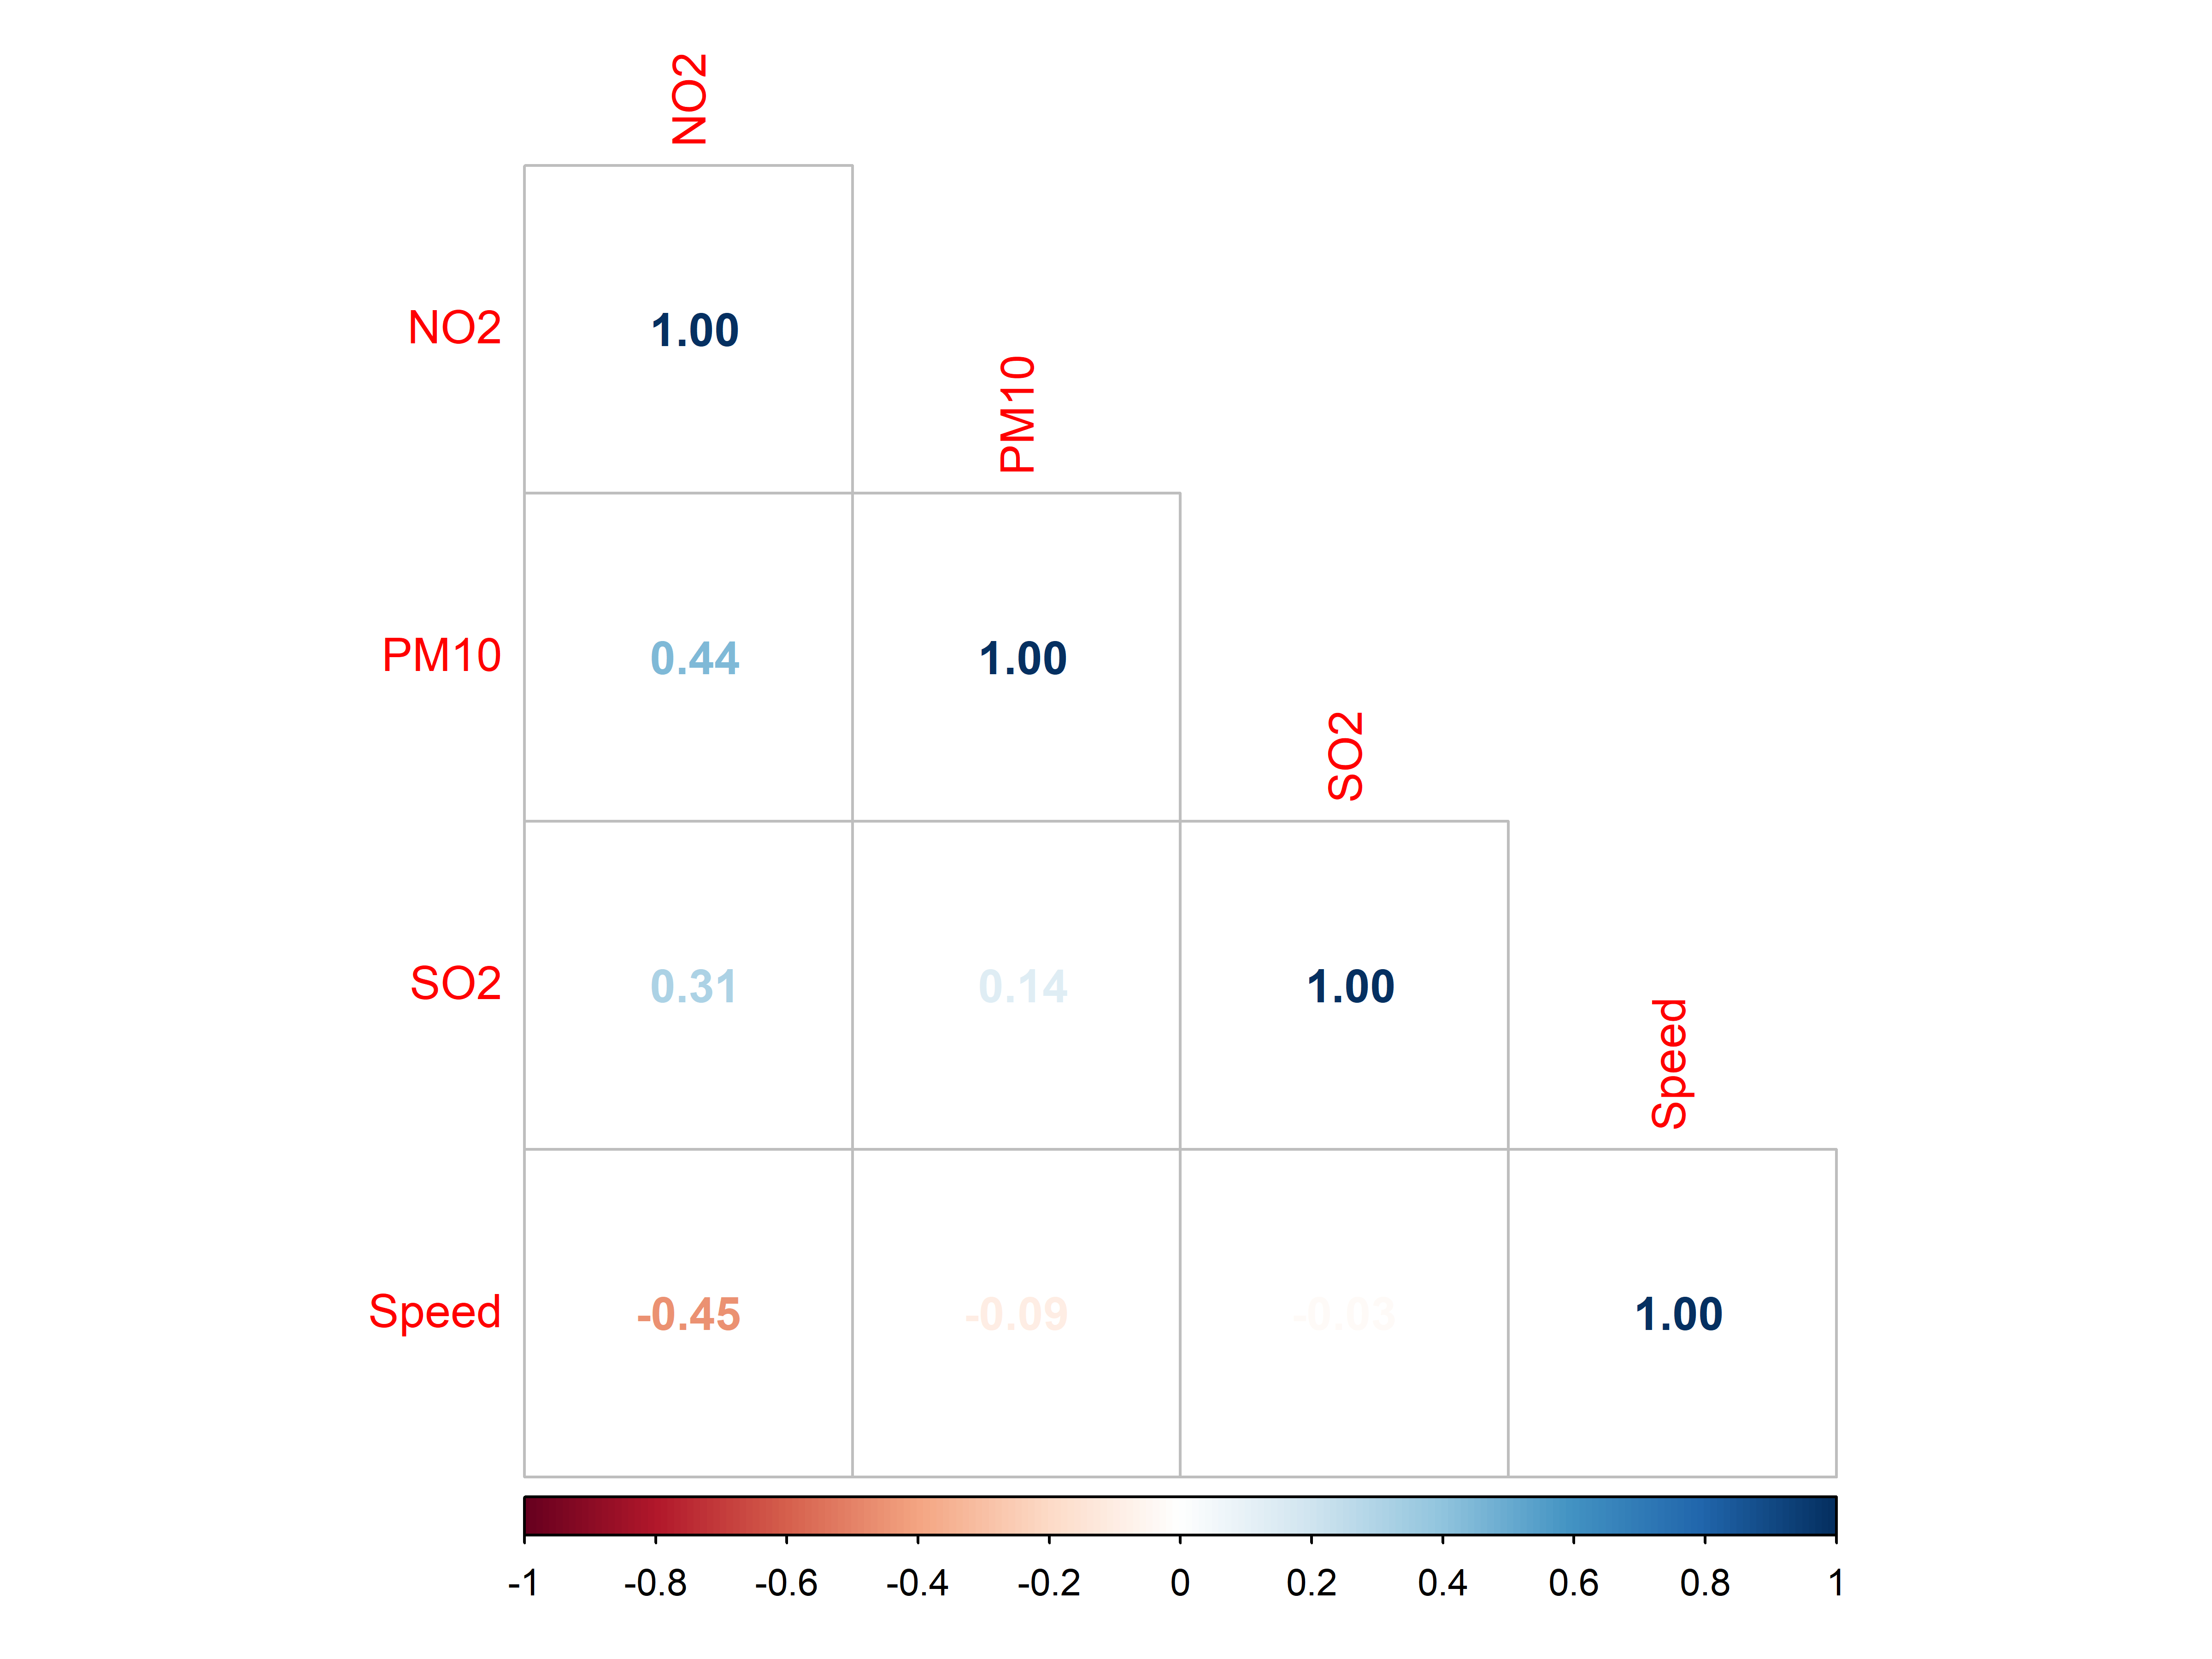
\includegraphics[width=0.48\linewidth]{../images/corrplot_2019.png}
         \caption{Correlation plot of the variables.}
      \end{figure}

      Our response variable $\text{NO}_{2}$ appears to be moderately positively correlated with $\text{PM}_{10}$ and $\text{SO}_{2}$, and moderately negatively correlated with Speed. These are not ideal explanatory variables since we typically would like them to be strongly correlated with the response variable. The explanatory variables are weekly correlated with one another, whether it be positive or negative correlation. This is ideal since some models do not work well with correlated explanatory variables, often leading to unstable point estimates and inflated standard errors.

      \vspace{1em}

      Before looking at the data. The proposed model for the mean function is $f(x_{t}) = x_{t}^{T} \beta + e$ and $g(x_{i}, x_{j}) = \alpha^{2} \text{exp}(- \frac{1}{2} (\frac{|x_i - x_j|}{\rho})^2) + \sigma\delta_{ij} \, \text{for} \, i,j \in \mathcal{I}$ for the covariance function. This allows us to capture the trend (if it exists) in the time series. This also allows us to model the correlation structure of the data. The squared exponential kernel is chosen because it is a natural way of describing the correlation decay.

      \begin{figure}[H]
         \centering
         \begin{subfigure}[t]{0.48\linewidth}
            \centering
            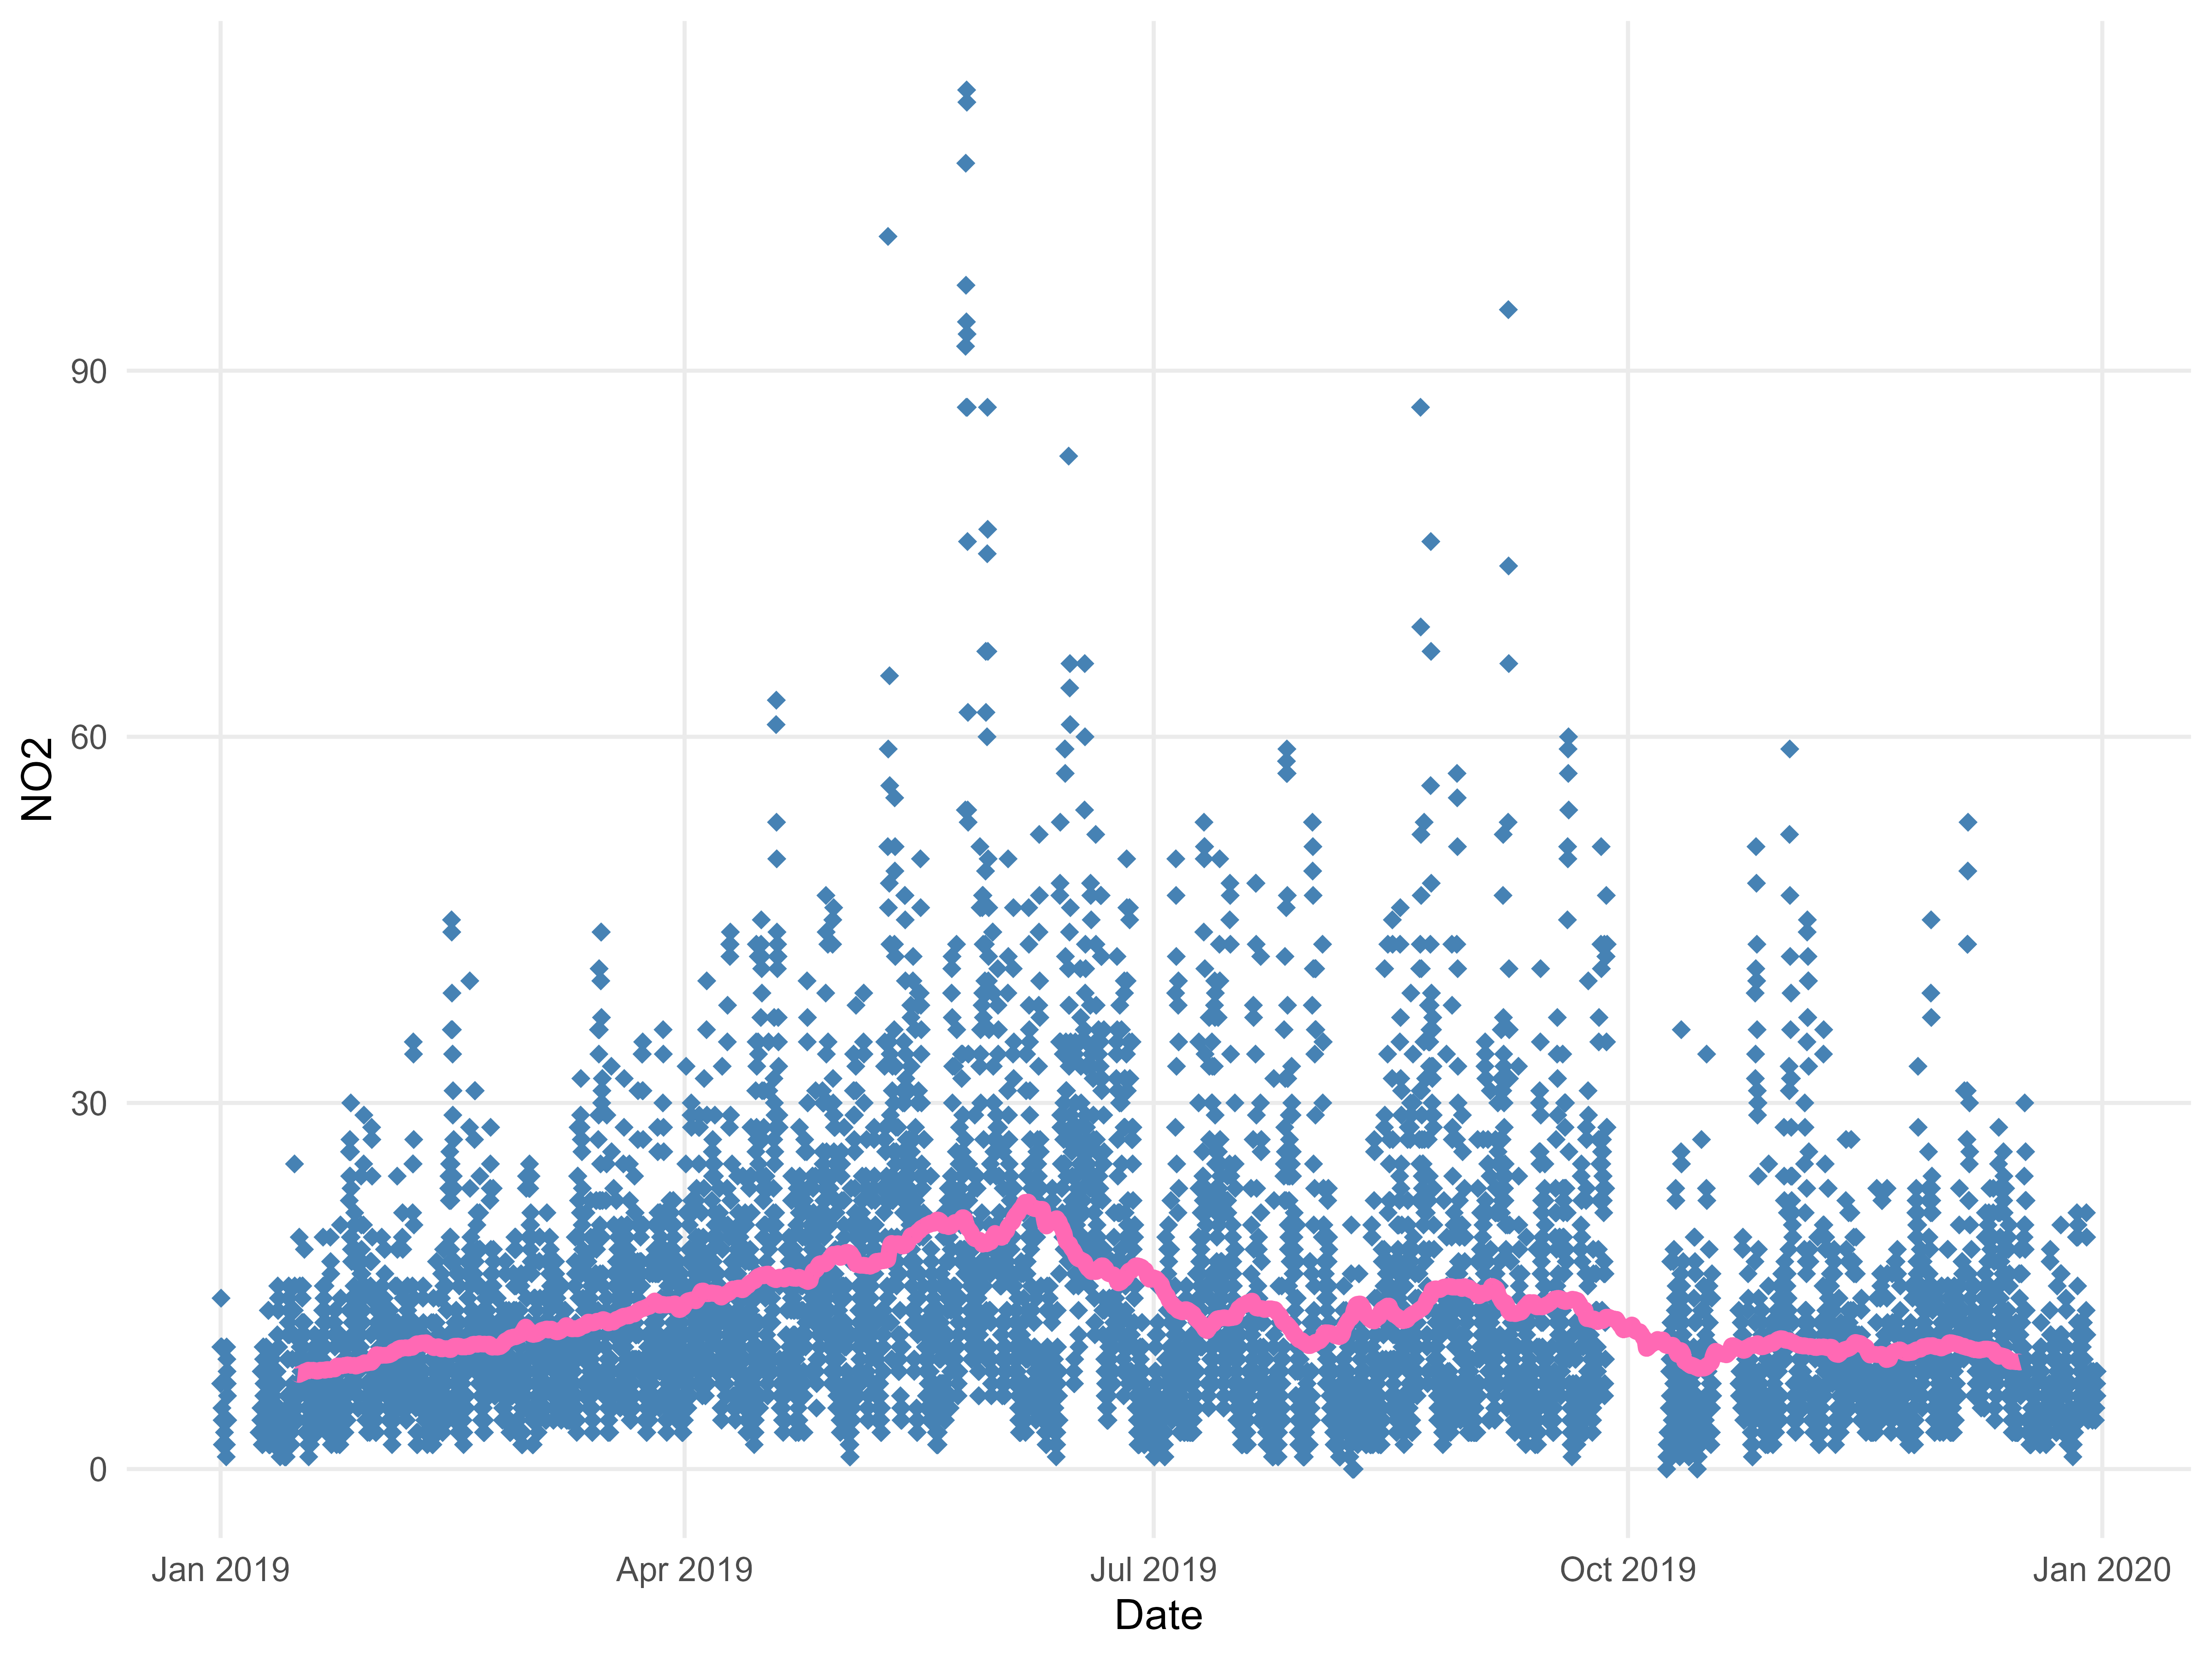
\includegraphics[width=\linewidth]{../images/no2_scatter_2019.png}
         \end{subfigure}
         \hfill
         \begin{subfigure}[t]{0.48\linewidth}
            \centering
            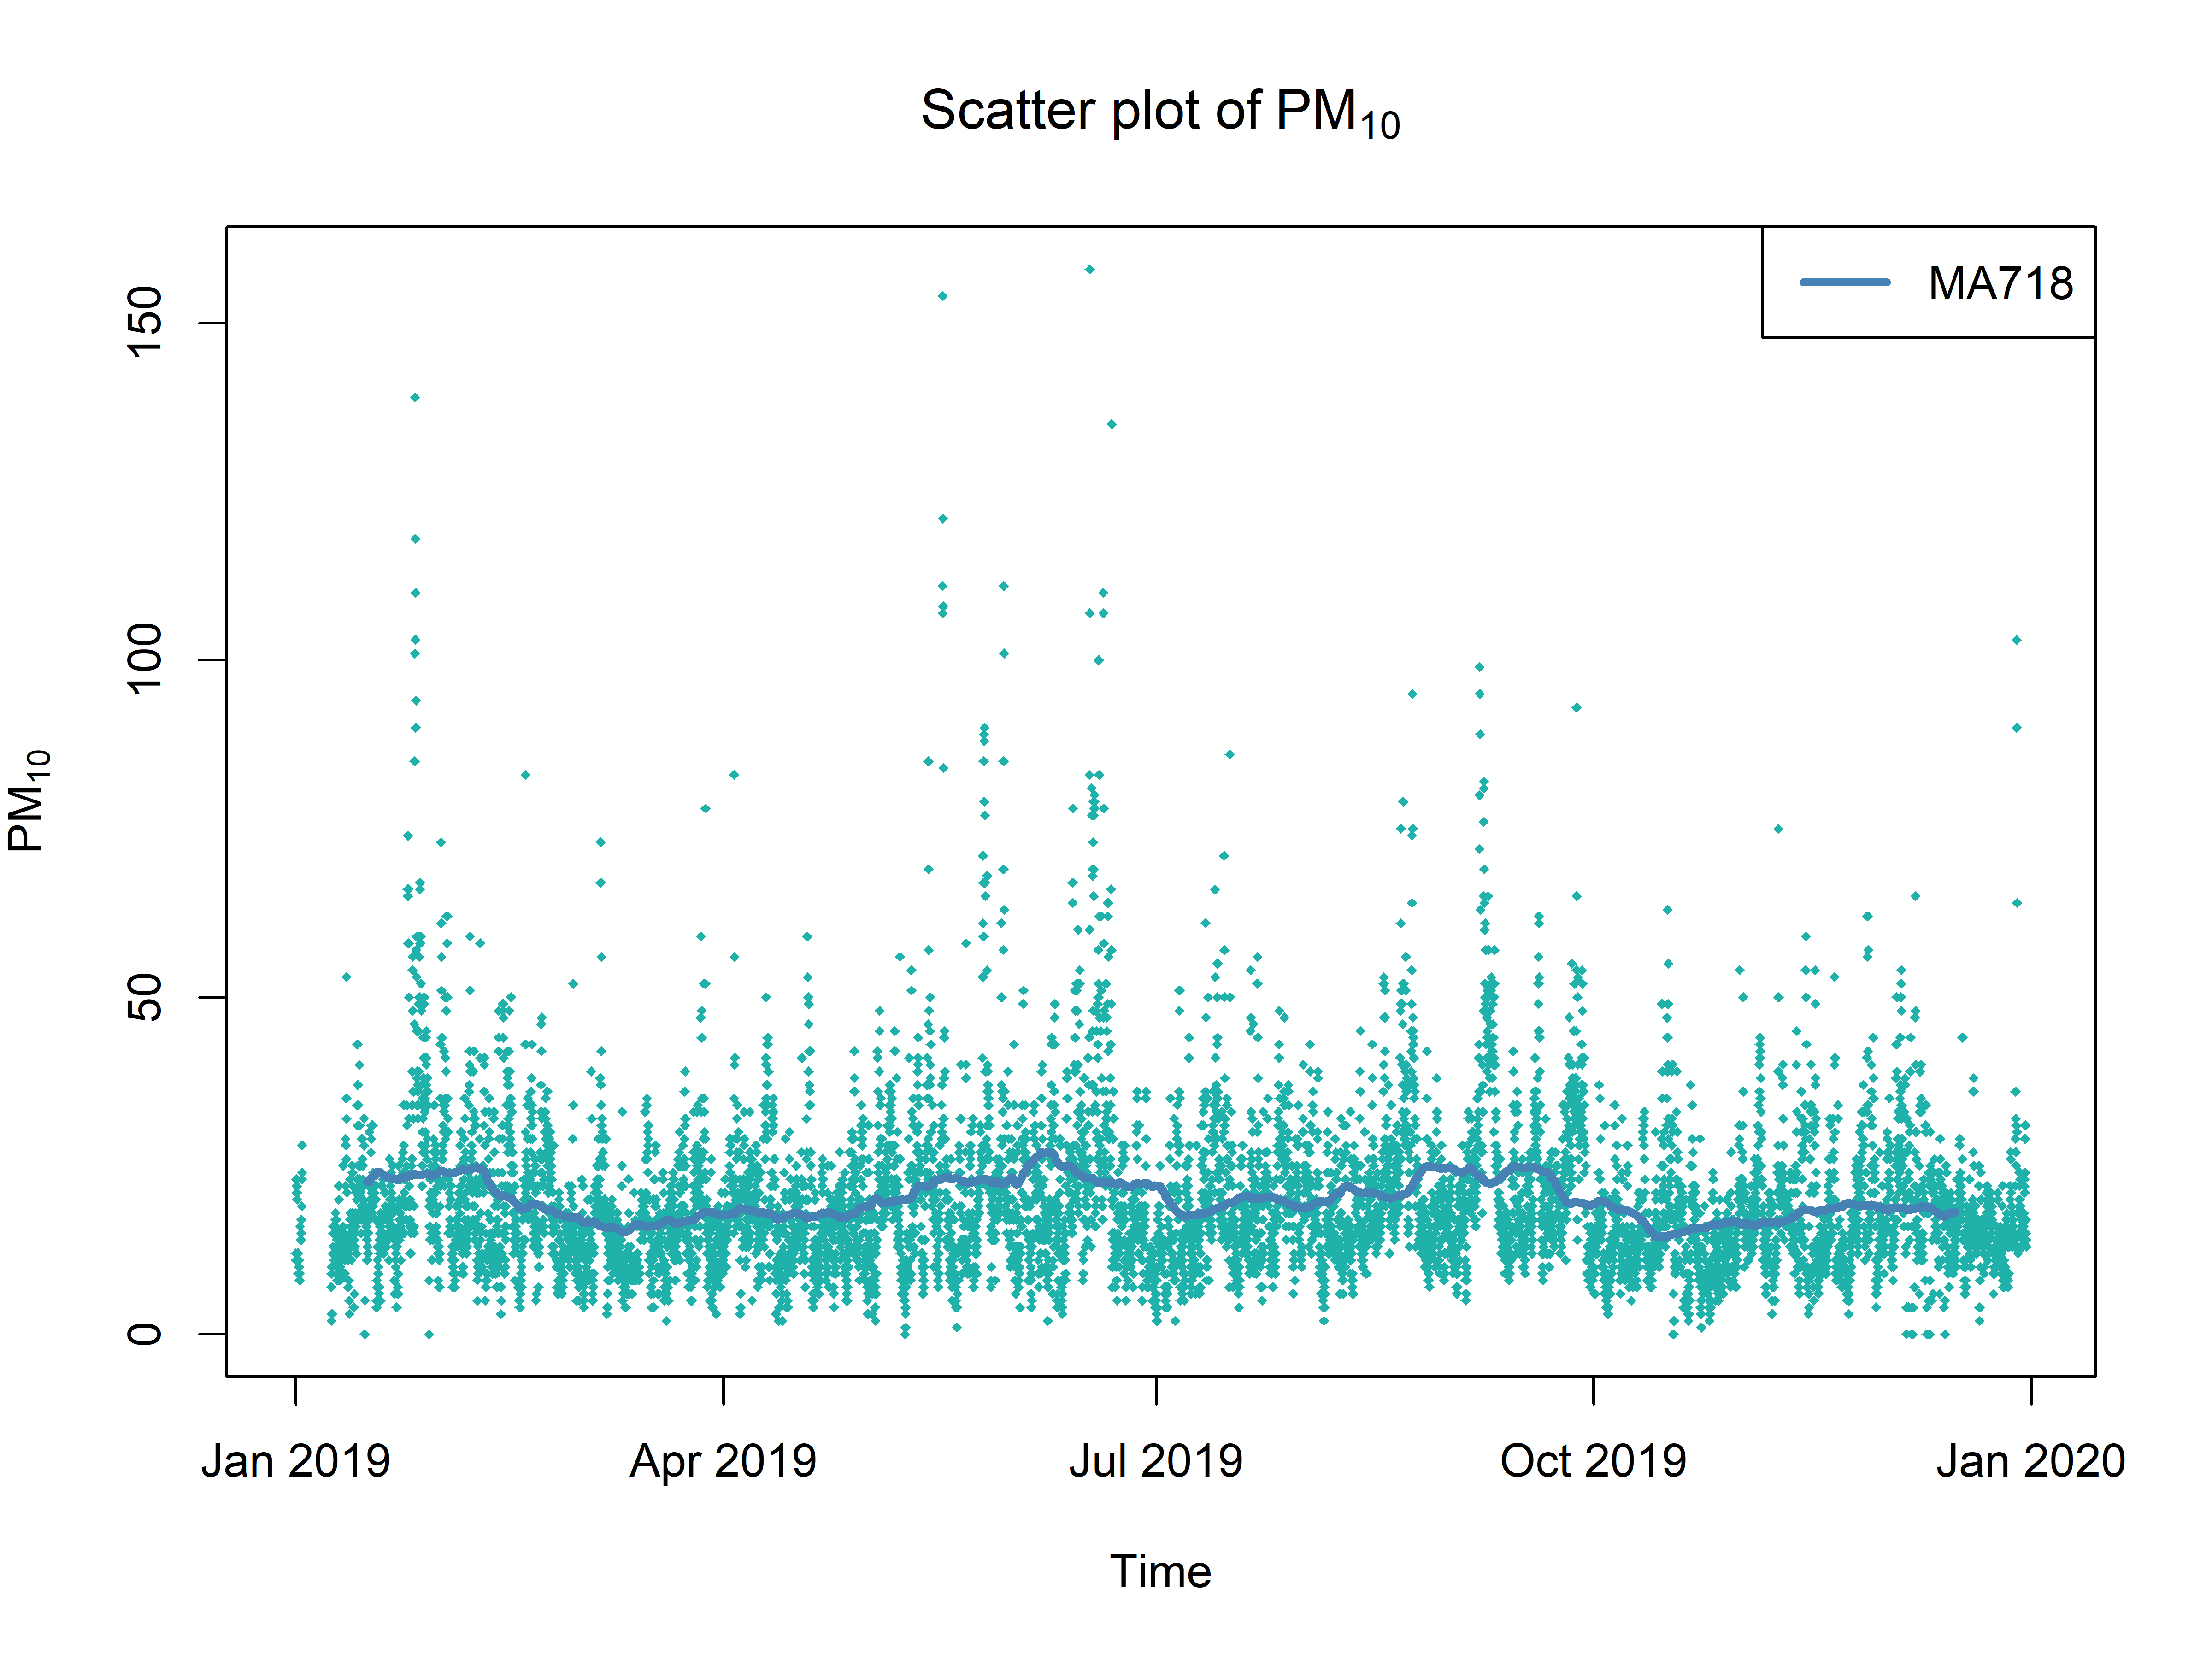
\includegraphics[width=\linewidth]{../images/pm10_scatter_2019.png}
         \end{subfigure}

         \vfill

         \begin{subfigure}[t]{0.48\linewidth}
            \centering
            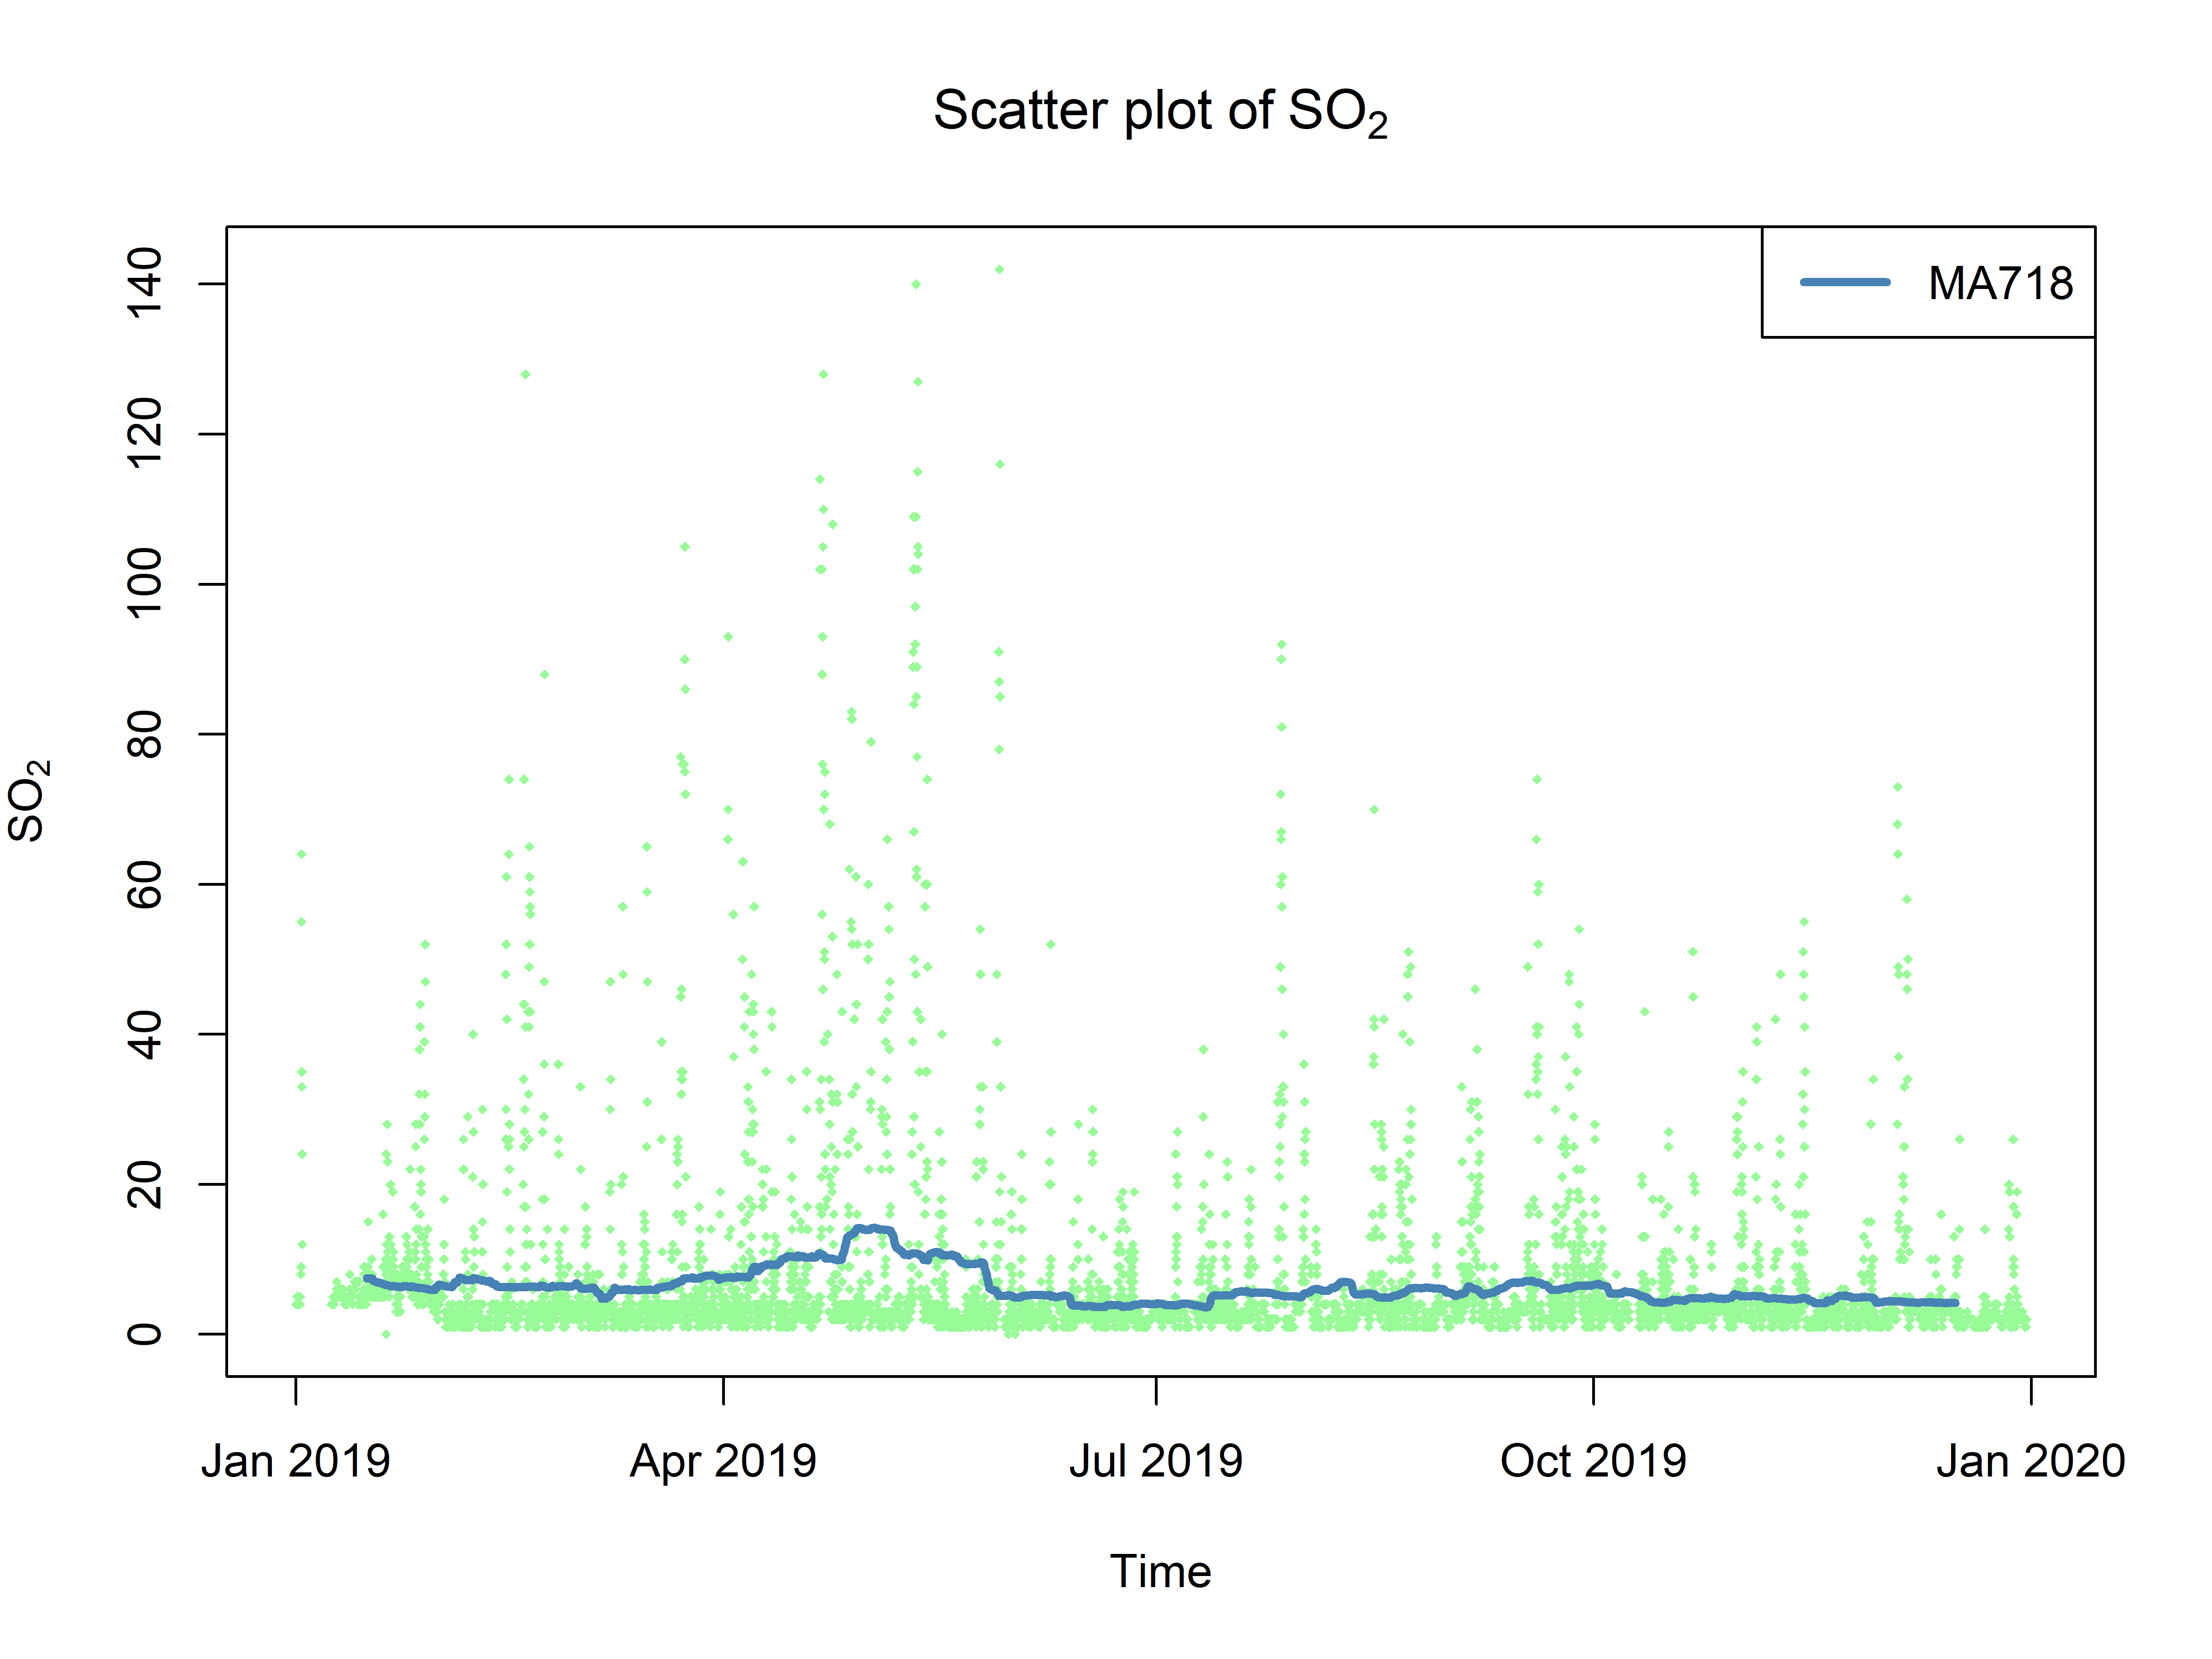
\includegraphics[width=\linewidth]{../images/so2_scatter_2019.png}
         \end{subfigure}
         \hfill
         \begin{subfigure}[t]{0.48\linewidth}
            \centering
            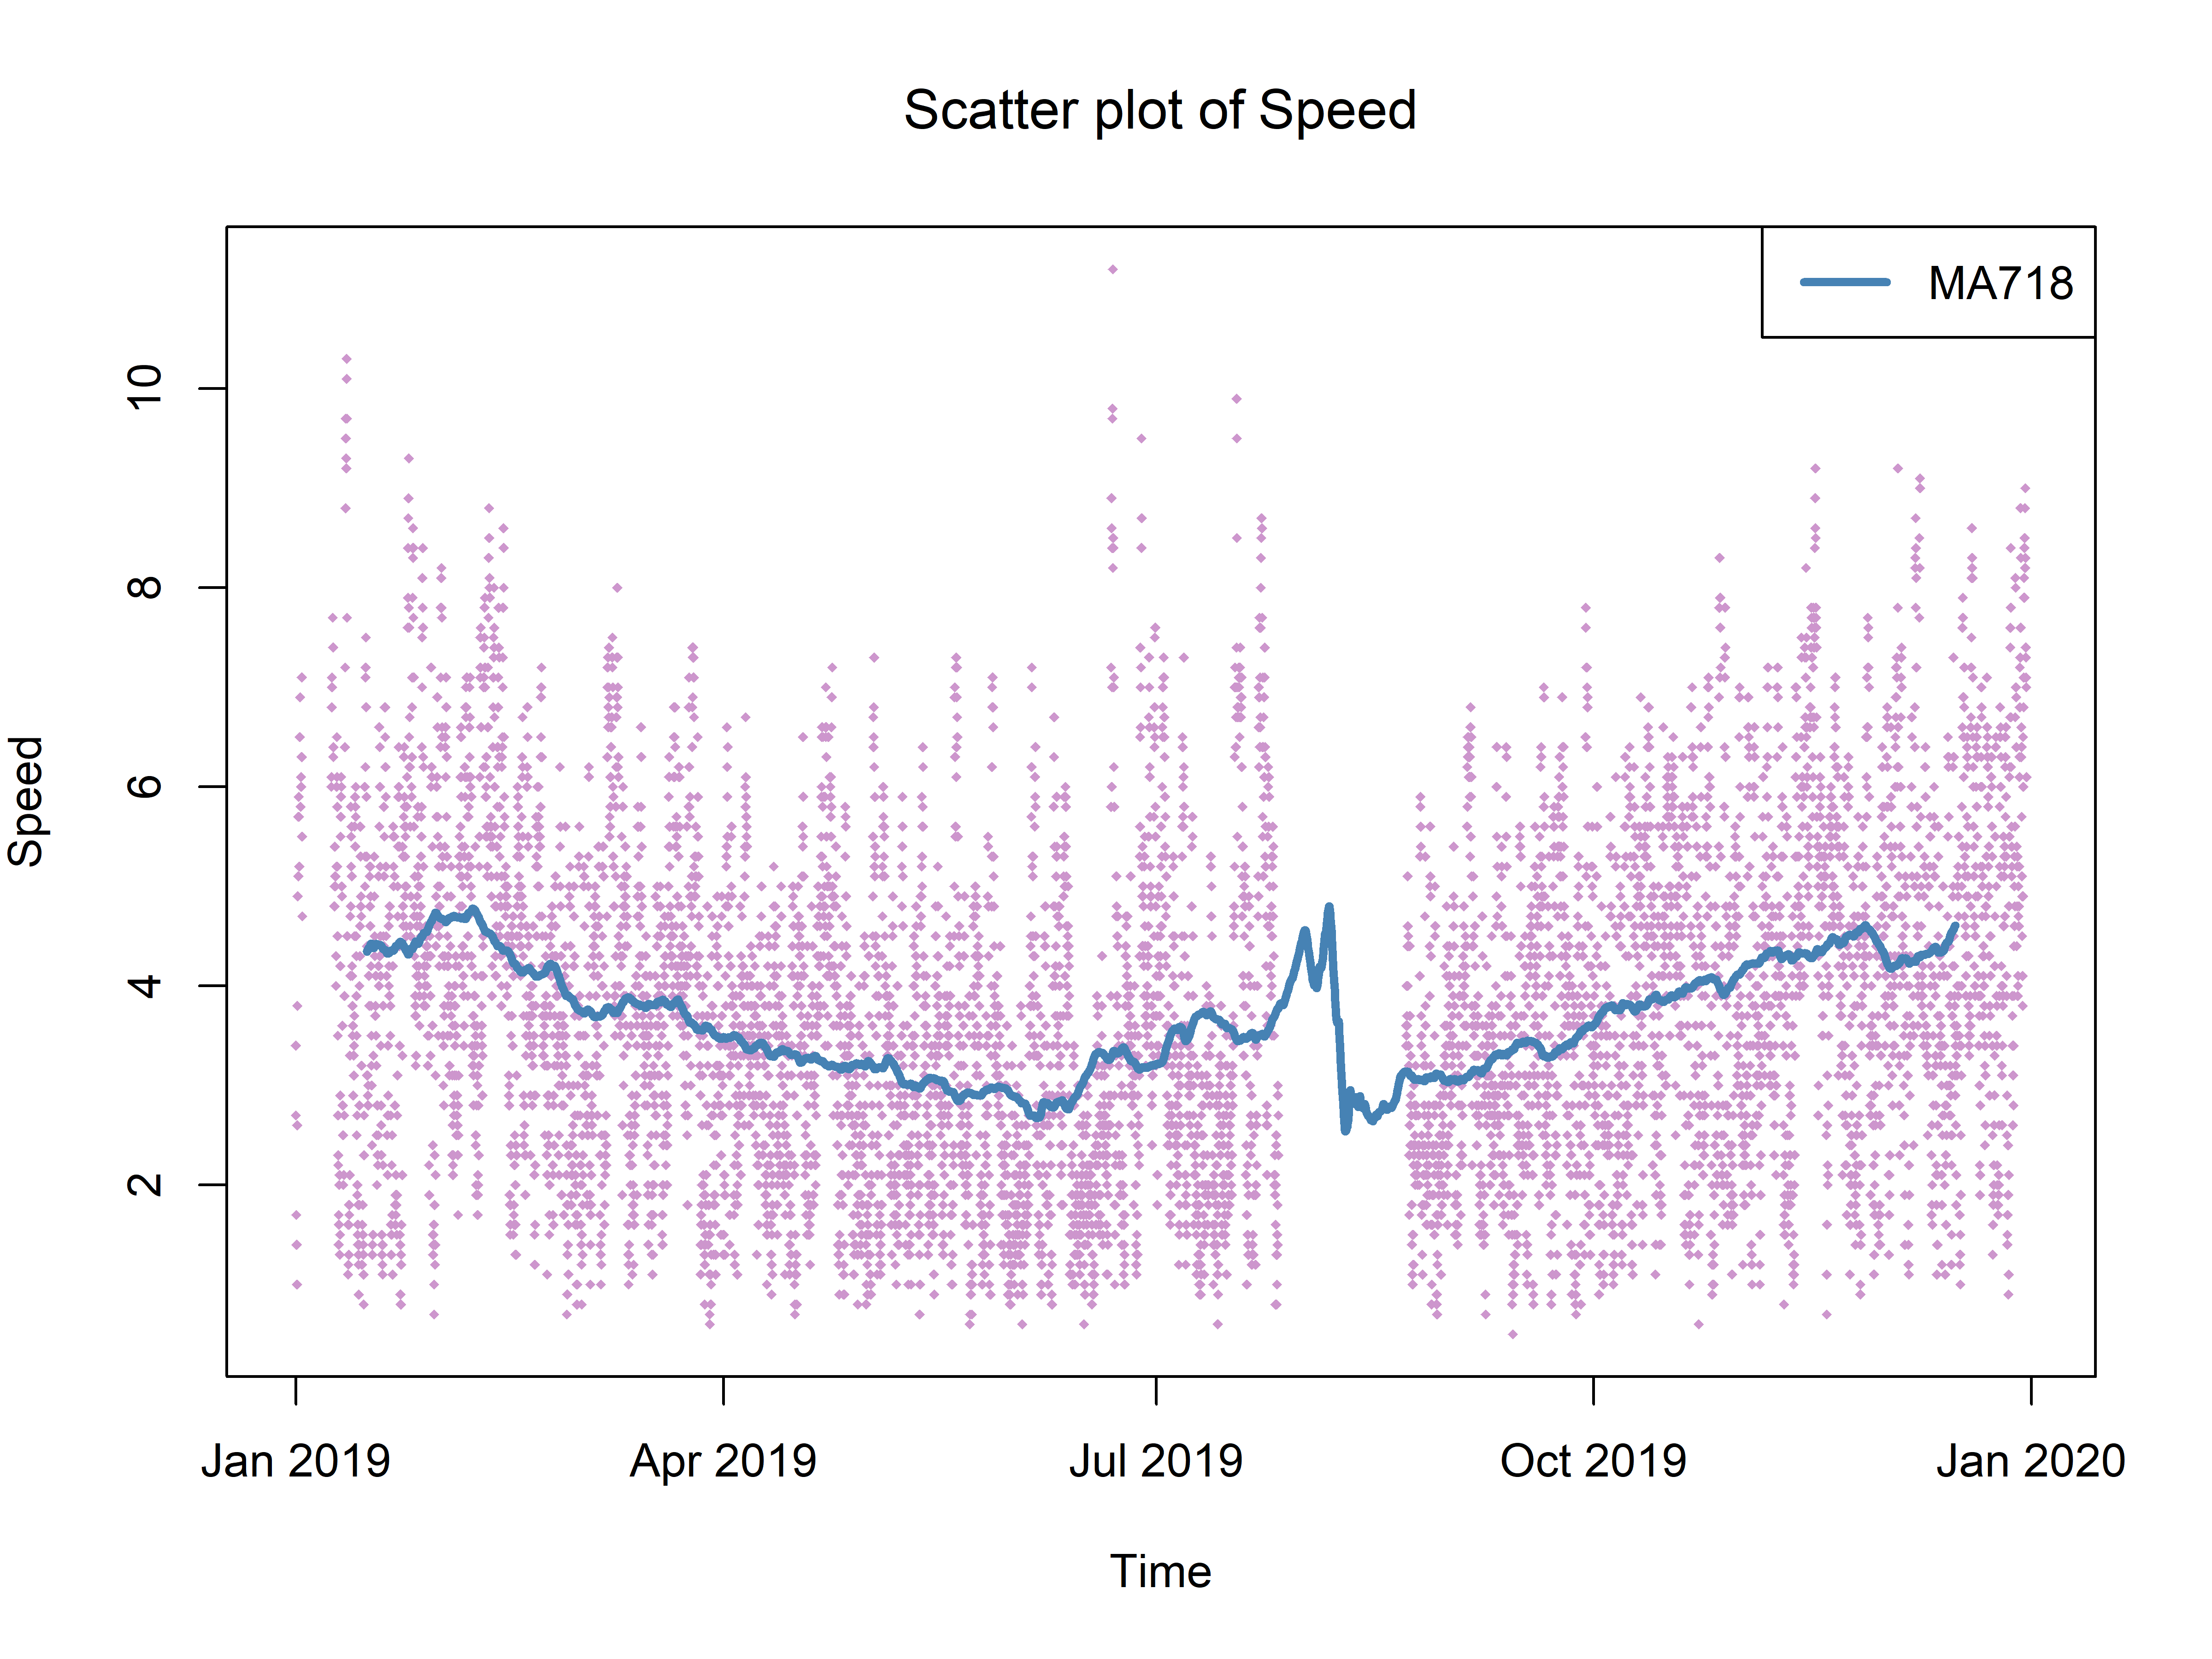
\includegraphics[width=\linewidth]{../images/speed_scatter_2019.png}
         \end{subfigure}
      \end{figure}


      \begin{figure}[H]
         \centering
         \begin{subfigure}[t]{0.48\linewidth}
            \centering
            
\includegraphics[width=\linewidth]{../images/no2_hist_2019.png}
         \end{subfigure}
         \hfill
         \begin{subfigure}[t]{0.48\linewidth}
            \centering
            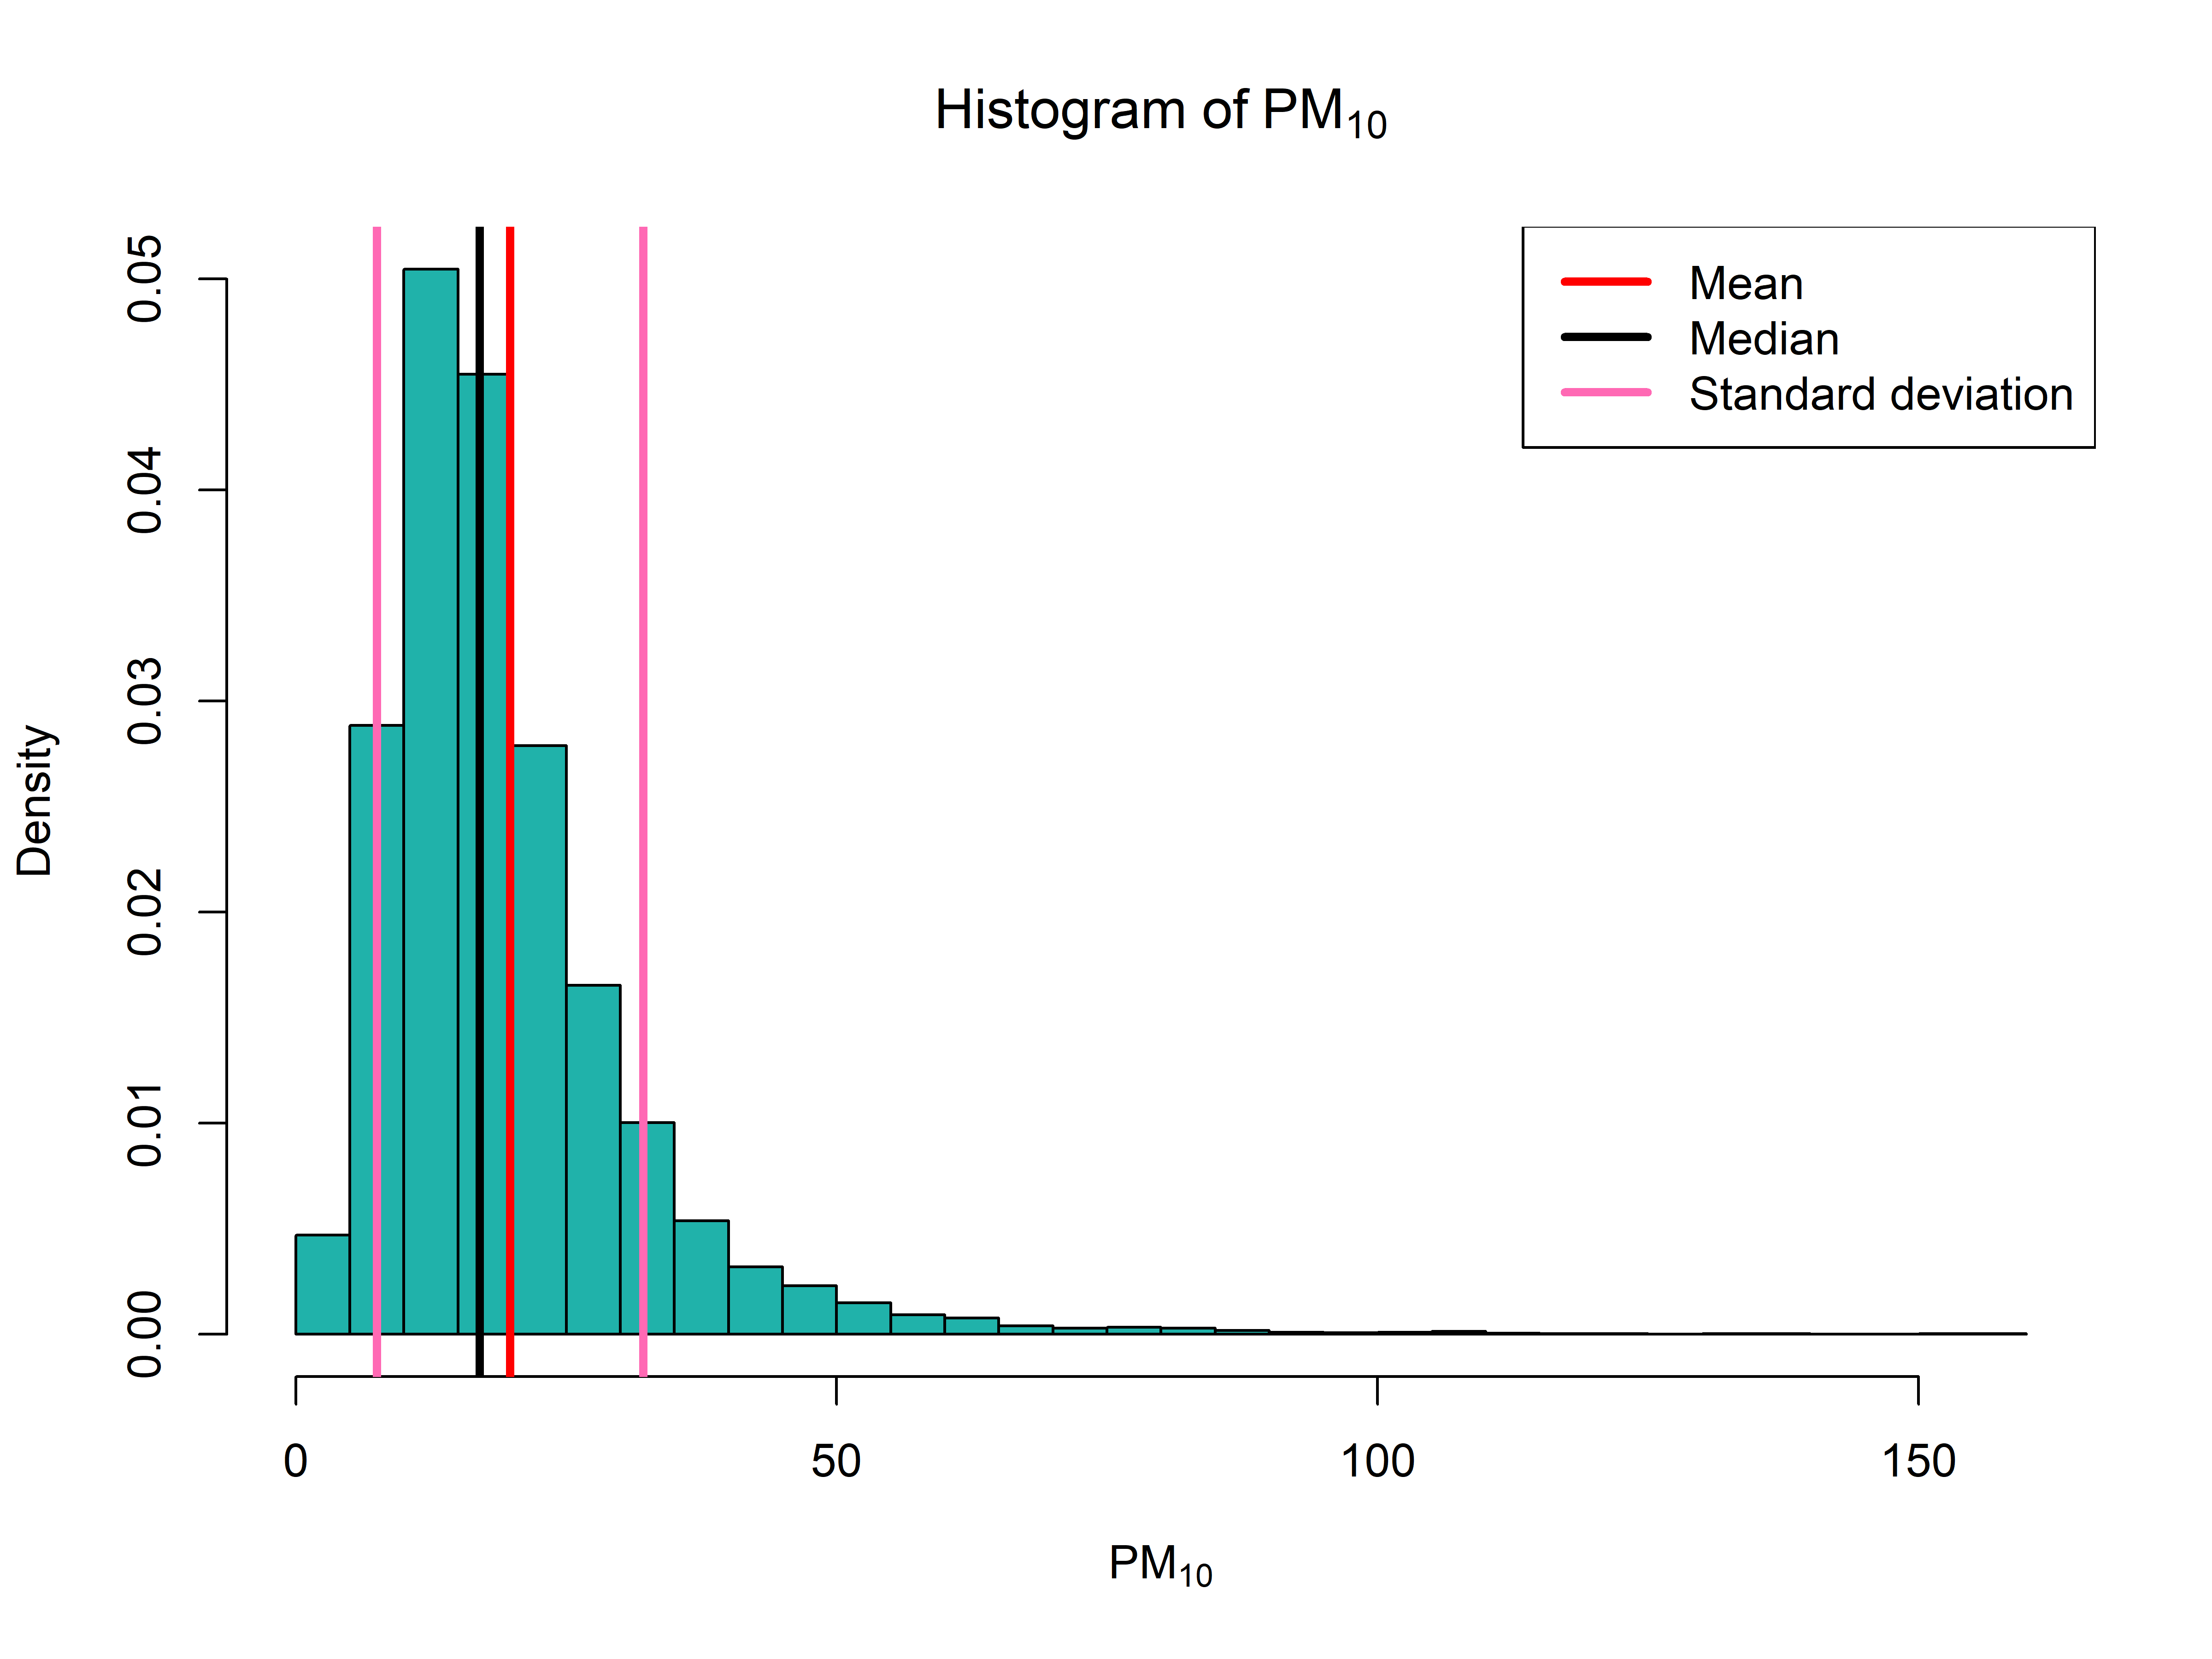
\includegraphics[width=\linewidth]{../images/pm10_hist_2019.png}
         \end{subfigure}

         \vfill

         \begin{subfigure}[t]{0.48\linewidth}
            \centering
            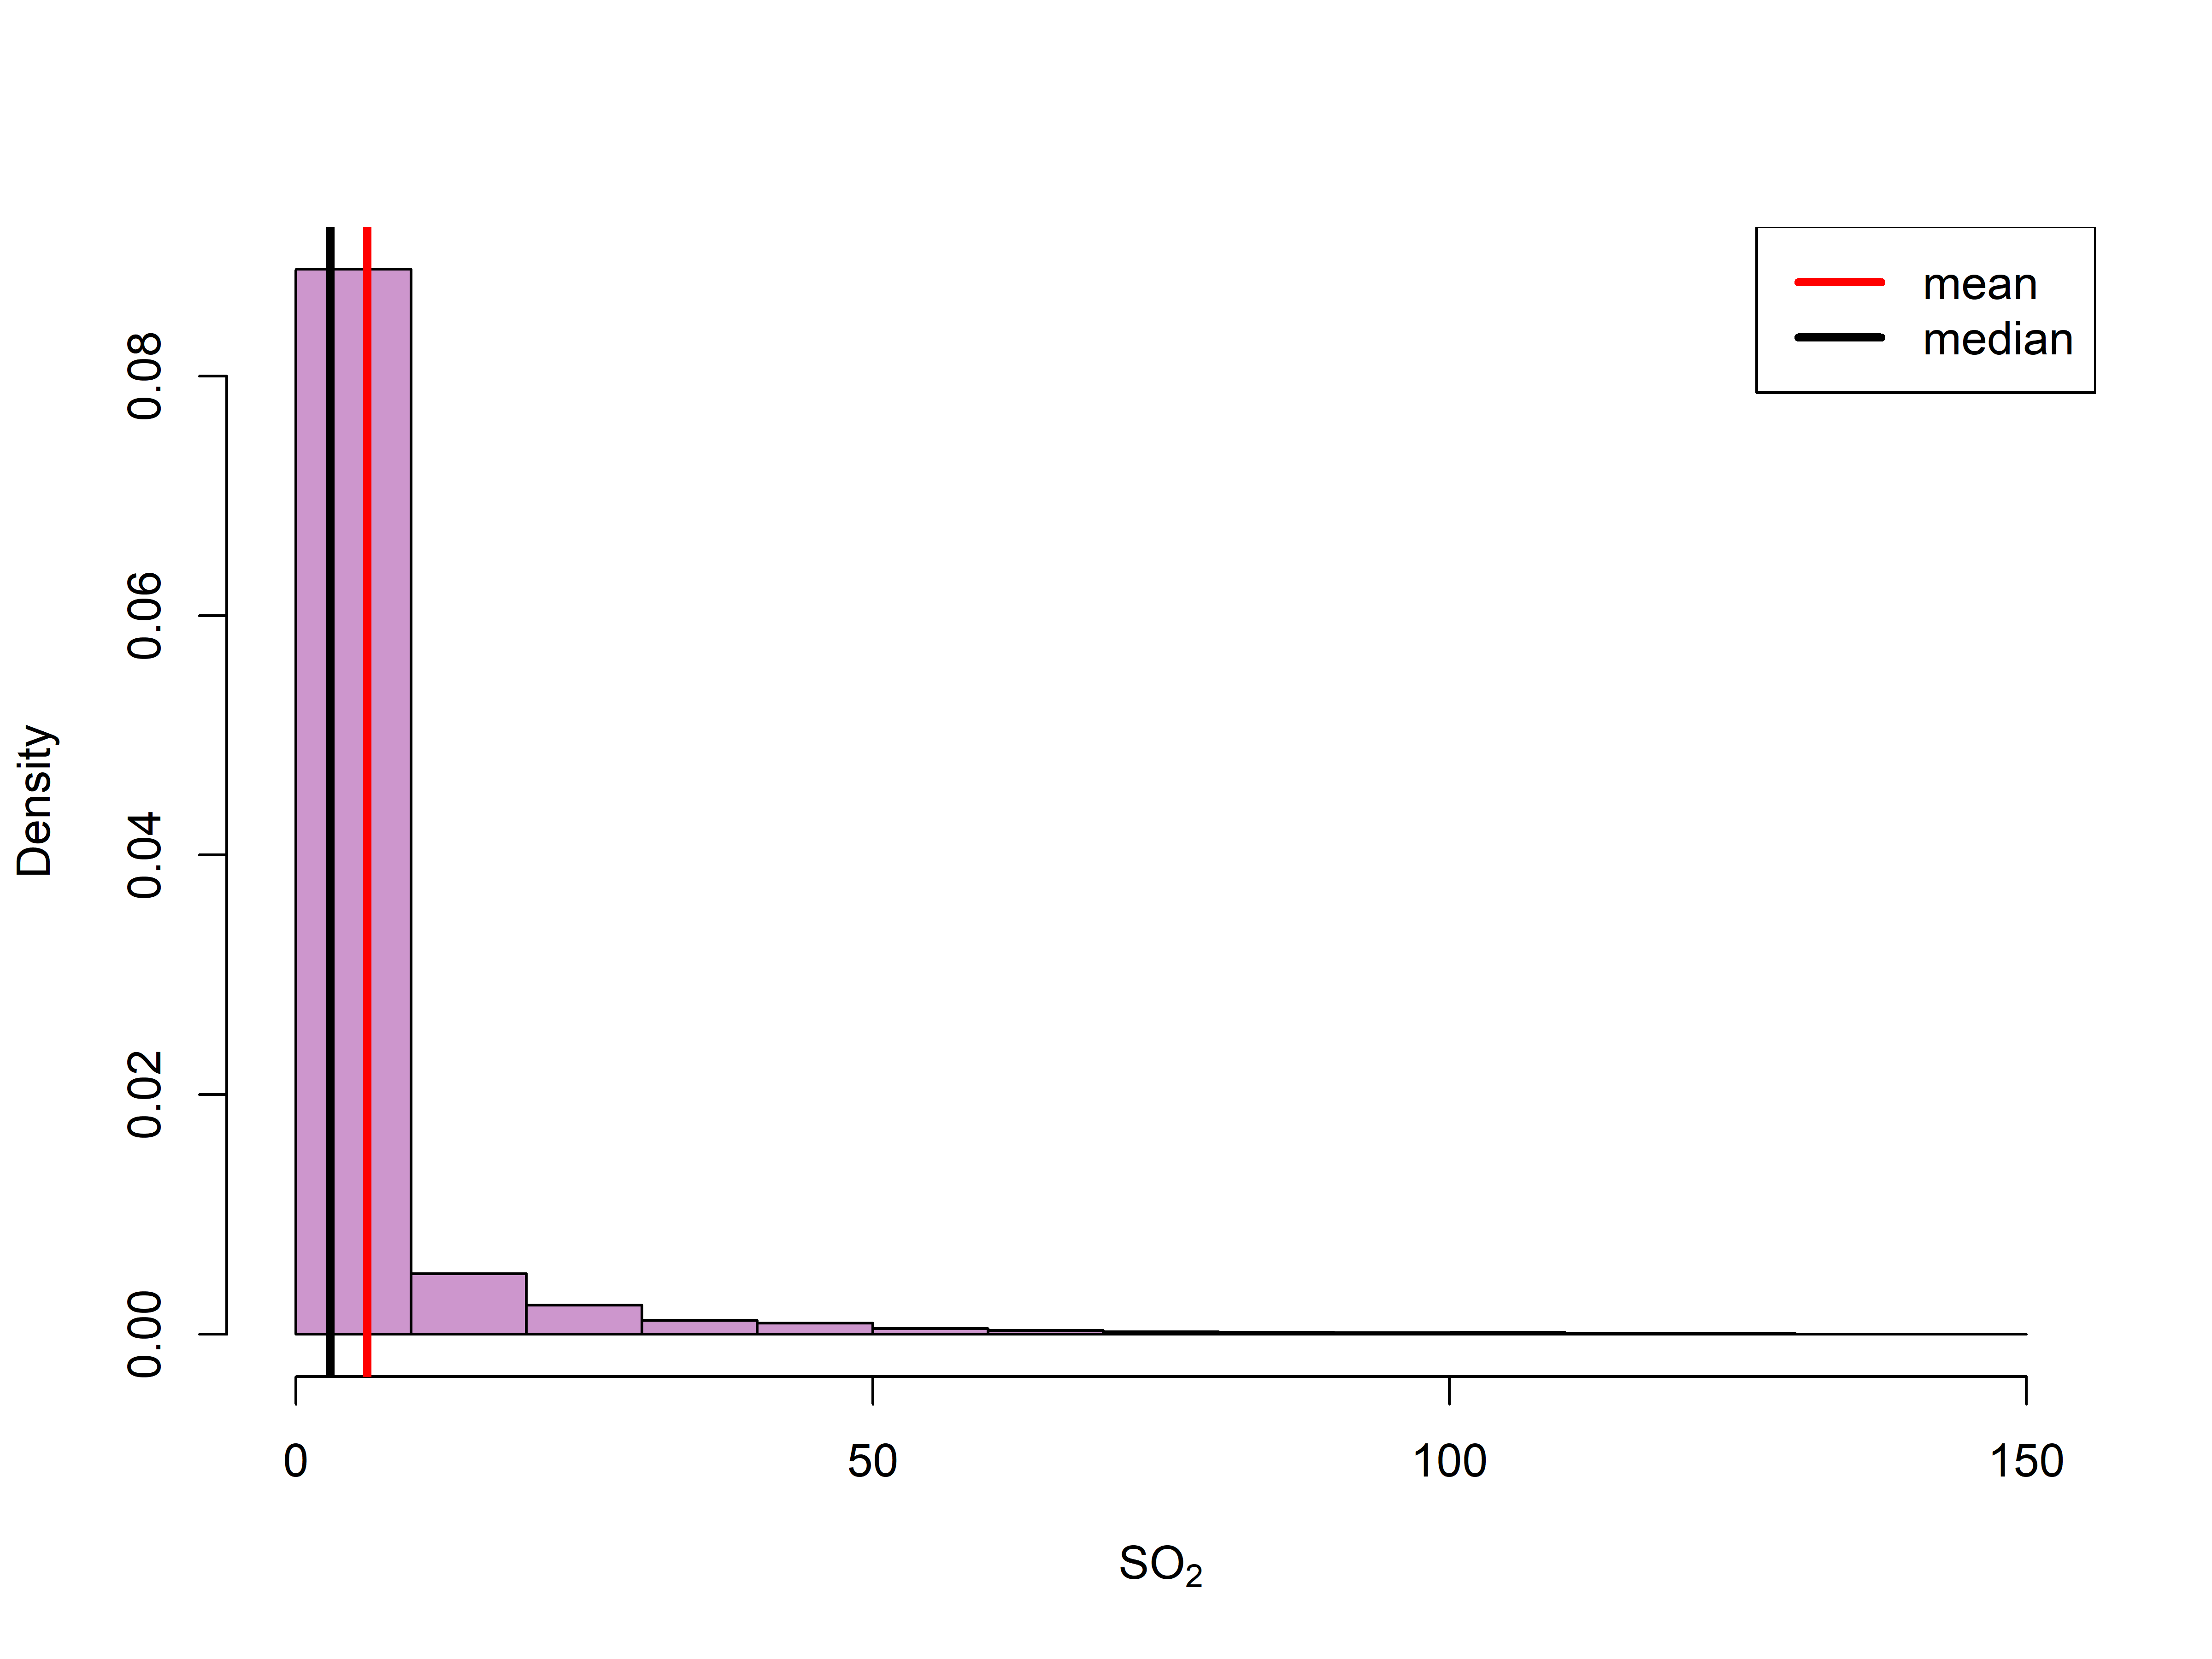
\includegraphics[width=\linewidth]{../images/so2_hist_2019.png}
         \end{subfigure}
         \hfill
         \begin{subfigure}[t]{0.48\linewidth}
            \centering
            
\includegraphics[width=\linewidth]{../images/speed_hist_2019.png}
         \end{subfigure}
      \end{figure}

      The mean appears to be constant, but the variance seems to be changing with time. Thus it is better if $f(x) = 0$ and $g(x) = \alpha^{2} \text{exp}(- \frac{1}{2} (\frac{|x_i - x_j|}{\rho})^2)$. The prior distributions of the exponantiated quadratic kernel are the following: $\alpha \sim \text{half-normal}(0, 1)$, $\rho \sim \mathcal{IG}(20, 10)$, and $\sigma \sim \text{half-normal}(0, 1)$. There is seasonality since regular patterns repeat for the seasons of the year. Random variation is present. However, there is no cyclical component present.
   
   \section*{References}
      \begin{enumerate}
         \item https://www.lung.org/clean-air/outdoors/what-makes-air-unhealthy/nitrogen-dioxide
      \end{enumerate}
   
   \end{flushleft}
\end{document}
